\documentclass[a4paper,12pt]{report}

\usepackage{graphicx}
\usepackage{amsmath}
\usepackage{hyperref}
\usepackage{enumitem}
\usepackage{amsmath}
\usepackage{amssymb}
\usepackage{subcaption}
\usepackage{float}

% Hyperref setup to avoid red boxes
\hypersetup{
    colorlinks=true,
    linkcolor=blue,
    filecolor=magenta,      
    urlcolor=cyan,
    pdftitle={Polyp Detection in Endoscopic Colonoscopy Frames using DeepLabV3+},
    bookmarks=true,
    pdfpagemode=FullScreen,
}

\begin{document}

\title{}
\begin{center}
\thispagestyle{empty}
 
\includegraphics[scale=0.085]{logo.pdf}\\*
\Large\bfseries{Indian Institute of Technology Roorkee}\\*
\vspace{1.5cm}
\end{center}
\begin{center}
\Large\bfseries{Project Report}
\end{center}
\begin{center}
\textit{on}
\end{center}
\begin{center}
\Large\bfseries{Polyp Detection in Endoscopic Colonoscopy Frames using DeepLabV3+}
\end{center}
\begin{center}
\textit{Submitted by}
\end{center}
\begin{center}
\Large\bfseries{Neha Sharma}\\*
\end{center}
\begin{center}
\textit{under the supervision of}\\
\Large\bfseries{Prof. Dr.  Millie Pant}\\
\end{center}
\begin{center}
\textit{Applied Mathematics and Scientific Computing, IIT Roorkee}\\
\end{center}
\begin{center}
 %\includegraphics[scale=2.3]{srm_logo.png}\\*
\Large\bfseries{Duration: 1/07/2025 – 15/08/2025 }\\*
\end{center}


\chapter*{Acknowledgements}
\thispagestyle{empty}

I am grateful for the opportunity to pursue my internship at the Department of Applied Mathematics and Scientific Computing, IIT Roorkee, under the guidance of Prof. Dr. Millie Pant, Head of Department. I extend my heartfelt thanks to Prof. Dr. Millie Pant for her constant support, encouragement, and insightful guidance, which created a rich learning environment and greatly enhanced my academic and professional development. Her leadership and vision made this internship a highly rewarding experience.\newline I would also like to sincerely thank Shubham Joshi sir for his valuable guidance and constructive advice during the course of my internship. His thoughtful feedback not only helped me refine my skills and problem‑solving approach but also kept me motivated to perform better. I am deeply appreciative of the time, effort, and encouragement he dedicated to helping me grow throughout this journey.

\clearpage


\begin{abstract}
Timely identification of colorectal polyps plays a crucial role in reducing the risk of colorectal cancer; however, manual segmentation during colonoscopies is often difficult because of the diverse appearance of polyps and inconsistencies in image quality. In this project, an advanced DeepLabV3+ based model is utilized to automate the segmentation of polyps in colonoscopy images taken from Kaggle. The methodology covers a comprehensive pipeline, starting from preprocessing and data augmentation to model training and careful adjustment of hyperparameters to maximize both accuracy and adaptability. Model performance was evaluated through metrics such as the Dice Coefficient and Intersection over Union (IoU), all of which indicated high segmentation reliability. To further enhance interpretability, Grad-CAM visualizations were employed, depicting explainability of the deep learning models. Overall, the results indicate that this approach not only delivers precise segmentation but also holds strong promise for real-time implementation. This advancement stands to support clinicians with a trustworthy tool for more effective early detection and intervention in colorectal cancer screening.
\end{abstract}

\tableofcontents
\newpage

\chapter{Introduction}
    \section{Background on Colorectal Cancer and Polyp Detection}
  Colorectal cancer is one of the most dangerous cancers worldwide and continues to be a major reason for illness and mortality across populations. In most cases, the disease begins with the formation of small, initially harmless growths known as polyps along the lining of the colon. While benign in their early stage, these polyps carry the risk of gradually developing into malignant tumors if left untreated. Detecting and removing them at an early stage is therefore one of the most effective strategies for reducing the chances of colorectal cancer.
Colonoscopy remains the standard method for screening and prevention, but its effectiveness largely depends on the endoscopist’s ability to carefully spot these growths in real time. Polyps, however, are highly variable—they can differ in size, shape, color, and even surface texture. Such diversity, combined with practical challenges like inadequate bowel cleansing, or poor lighting during the procedure, makes them easy to miss. As a result, a significant number of polyps go undetected during routine screenings, highlighting the urgent need for more reliable and supportive detection methods.


    \subsection{Symptoms and Progression}
    \textbf{Early Stage Symptoms:}
Colorectal cancer often starts silently. Early signs, if any, are subtle—slight bowel changes, small amounts of rectal bleeding, or mild stomach discomfort. Most polyps cause no symptoms, making regular screening the only reliable way to catch them early.\\
{}
\newline\textbf{Progressive Symptoms:}
As cancer grows, symptoms become harder to ignore such as ongoing bowel habit changes, visible blood in stool, stomach pain or cramps, weight loss, fatigue, and the feeling of not fully emptying the bowel. These symptoms start to interfere with everyday life.\\
{}
\newline\textbf{Disease Progression Stages:}
\begin{itemize}
    \item Stage 0–I: Cancer stays within the bowel wall, minimal symptoms.
    \item Stage II–III: Spreads deeper and into lymph nodes, symptoms get worse.
    \item Stage IV: Reaches distant organs—causing issues like jaundice (liver) or breathing problems (lungs).
\end{itemize}


    \subsection{Pathophysiology}
Colorectal polyps begins to grow when genetic mutations disrupt the normal control of cell growth, leading to small tissue outgrowths along the colon lining. Over time, these polyps can undergo a process known as the adenoma–carcinoma sequence. This sequence is driven by stepwise molecular changes—starting with mutations in the APC gene, followed by K-ras activation, and later p53 inactivation. Together, these changes push cells from harmless growths toward malignant tumors. Recognizing this chain of events shows why identifying and removing polyps early is very important in preventing colorectal cancer.
  
    \subsection{Risk Factors}
\begin{enumerate}
    \item\textbf{Age:} The risk of developing colorectal cancer goes up as people get older. Most cases are found in individuals over 50, and the likelihood continues to increase with advancing age due to long-term exposure to genetic and environmental factors.
    \item\textbf{Genetics:} Family history plays a big role. Having a close relative (parent, sibling, or child) with colorectal cancer or advanced polyps raises the risk. The risk is even higher if more than one family member is affected or if the cancer appeared at an early age.
    \item\textbf{Lifestyle Factors:} Unhealthy habits such as being overweight, not getting enough physical activity, smoking, and heavy alcohol consumption all add to the risk. These factors trigger cancer development through changes like insulin resistance, chronic inflammation, and exposure to harmful substances.
    \item\textbf{Diet:} High intake of red and processed meats, high-temperature cooking, and low fiber, fruit, and vegetable consumption are linked to higher risk, while balanced, plant-forward diets are protective.
 \end{enumerate}

    \subsection{Current Diagnosis Methods}
Standard diagnostic approaches include colonoscopy, CT colonography, fecal occult blood testing, and sigmoidoscopy. Colonoscopy remains the gold standard due to its dual diagnostic and therapeutic capability, allowing real-time polyp detection and removal during the same procedure.

    \subsection{Treatment and Management}
Current treatment involves endoscopic polyp removal (polypectomy) during colonoscopy, with follow-up surveillance based on polyp characteristics. Management protocols depend on polyp size, histology, and number, determining subsequent screening intervals and treatment strategies.
 \section{Importance of Early Detection}
    \subsection{Benefit of Early Detection}
Finding colorectal cancer early often means identifying and removing precancerous polyps, preventing cancer from developing. Early-stage detection enables less invasive treatments, lowers complication rates, and significantly improves survival, with markedly higher 5-year survival when localized. It also preserves quality of life by avoiding extensive chemotherapy or radiation and reduces healthcare costs through simpler, shorter therapies. Routine screening beginning in midlife maximizes these gains by catching disease before symptoms appear.
    \subsection{Detection Challenges}
\begin{enumerate}
    \item\textbf{Flat and sessile lesions:} These polyps are subtle, low-profile, and lack prominent protrusion, making them easy to miss on standard white-light endoscopy; enhanced imaging or dye-spray can help.
    \item\textbf{Inadequate bowel preparation:} Residual stool and fluid obscure mucosa, reducing visibility and polyp detection; rigorous prep instructions and split-dose regimens improve visualization.
    \item\textbf{Poor visualization conditions:} Folding anatomy, blind spots behind flexures, and rapid peristalsis limit view; dynamic position changes and water exchange techniques help expose mucosa.

 \end{enumerate}
    \subsection{Strategies for Early Detection}
Begin routine screening at 45 for average-risk adults; start earlier and screen more often for those with family history, hereditary syndromes, or inflammatory bowel disease. Use annual FIT as a simple, accurate stool test; consider stool DNA-FIT every 1–3 years for higher cancer sensitivity. Colonoscopy every 10 years remains the gold standard, enabling detection and removal of precancerous polyps in one procedure. Ensure programmatic follow-up: prompt diagnostic colonoscopy after positive tests and guideline-based surveillance. Optimize exam quality with split-dose bowel prep, adequate withdrawal time, high-definition imaging, and AI assistance. Offer CT colonography or colon capsule when colonoscopy is declined.



\section{Problem Statement and Hypothesis}
\subsection{Problem Statement}
Detecting polyps during a colonoscopy still depends a lot on the doctor’s eye and experience, which creates several challenges. Research shows that between 6\% and 27\% of polyps can be missed, and the rates vary widely between hospitals and doctors. Smaller polyps are tricky—they are easier to miss but are also important to catch early since they can develop into cancer over time. Longer procedures can also reduce accuracy because of fatigue and reduced focus. Differences in training and experience mean that detection rates can vary a lot from one gastroenterologist to another. Finally, because colonoscopy requires doctors to make decisions instantly in real time, the pressure can further impact accuracy. All these factors make consistent and reliable polyp detection difficult, highlighting the need for better supportive tools like automated segmentation.

\subsection{Hypothesis}
Deep learning models for semantic segmentation, such as DeepLabV3+ with a ResNet-50 backbone, can be highly effective in identifying polyps at the pixel level in colonoscopy images. Along with accurate segmentation, these models can also provide explainable outputs through attention or heatmap visualizations, helping doctors understand why the model made a certain prediction. The idea is that using such systems can lower polyp miss rates and make detection more consistent.


\subsection{Experiment Flowchart}

\begin{figure}[h]
    \centering
    \includegraphics[width=\textwidth]{flowchart.png}
    \caption{Experiment Flowchart}
    \label{fig:experiment_flowchart}
\end{figure}



    \section{Objectives of the Project}
    \subsection{Primary Objectives}
\begin{enumerate}
    \item\textbf{Automated Polyp Segmentation:}
    To build a reliable deep learning model that can automatically segment polyps in colonoscopy images with pixel-level accuracy, while meeting performance standards that are meaningful in real clinical practice.
    \item\textbf{Real-time Processing Capability:}
     Implement a system that can process colonoscopy images in real-time, suitable for integration into existing endoscopic equipment and clinical workflows.
    \item\textbf{Clinical Decision Support:}
     Create a comprehensive diagnostic tool that provides multiple visualization modalities to assist gastroenterologists in polyp identification and characterization.
 \end{enumerate}

    \subsection{Secondary Objectives}
\begin{enumerate}
    \item\textbf{Explainable AI Integration:}
     Implement interpretability techniques to provide transparent insights into model decision-making processes, enhancing trust and clinical adoption.
    \item\textbf{Multi-modal Visualization:}
       Develop comprehensive visualization tools including segmentation masks, probability heatmaps, attention maps, and bounding box detection to support different clinical use cases.
    \item\textbf{Performance Benchmarking:}
       Establish baseline performance metrics and conduct comparative analysis with existing polyp detection approaches.
 \end{enumerate}
    \subsection{Specific Goals}
    \begin{itemize}
    \item   Achieve IoU scores above 0.75 on validation datasets
    \item   Implement Grad-CAM visualization for model interpretability
    \item   Develop a user-friendly web interface for real-time inference
    \item   Create comprehensive documentation and clinical usage guidelines
    \item   Establish preprocessing pipelines that handle diverse image qualities and conditions
    \end{itemize}
    


    \section{Introduction to Deep Learning for Medical Imaging}
    Deep learning has revolutionized medical image analysis by enabling automatic feature extraction and pattern recognition that often surpasses traditional computer vision approaches. Convolutional Neural Networks (CNNs) have proven particularly effective for medical imaging tasks due to their ability to capture spatial hierarchies and local patterns crucial for diagnostic applications.
Semantic segmentation, the task of classifying every pixel in an image, represents a fundamental challenge in medical imaging where precise boundary delineation is essential. Unlike classification tasks that provide image-level predictions, segmentation enables pixel-level analysis crucial for surgical planning, disease monitoring, and treatment assessment.
The evolution from fully connected networks to convolutional architectures, and subsequently to advanced frameworks like DeepLabV3+, has enabled increasingly sophisticated medical image analysis capabilities. 

    \section{Applications of AI in Healthcare}
  
    \subsection{Medical Image Segmentation:}
        Medical image segmentation is widely used across different fields of healthcare, including radiology and pathology. In gastroenterology, it plays a key role by allowing accurate measurement of lesions, automated detection of polyps, and detailed analysis of mucosal irregularities. These tools provide consistent, objective data that support doctors in making decisions and give clinical judgment. 
    \subsection{Computer-Aided Diagnosis:}
   Computer-aided diagnosis (CAD) systems act as supportive tools to help doctors make faster and more accurate decisions. In colonoscopy, they can flag possible polyps in real time, mark areas that look suspicious, and provide measurable details about abnormalities. Rather than replacing the expertise of gastroenterologists, CAD systems are meant to help it—offering extra insights that strengthen evidence-based clinical decisions.
    \subsection{Real-time Screening Systems:}
Bringing AI into real-time screening is a major step forward in preventive healthcare. In colonoscopy, AI systems can give instant feedback during the procedure, helping doctors spot polyps that might otherwise be missed and improving the overall quality of screening. To be effective in practice, these systems need to deliver accurate results quickly, without slowing down the workflow of the procedure. 
    \subsection{Endoscopic Applications:}
   Endoscopic AI applications extend beyond polyp detection to include classification of lesion types, assessment of invasion depth, and prediction of histological characteristics. Advanced systems can provide multi-class segmentation, distinguishing between different tissue types and pathological conditions within a single procedure.

    \section{Motivation}
    The motivation for this project stems from converging factors in modern healthcare. The significant impact of colorectal cancer creates urgent need for improved screening technologies, as current polyp detection miss rates represent clear opportunities for technological intervention to improve patient outcomes. Advances in deep learning, particularly computer vision and medical imaging, have reached maturity levels enabling feasible and effective clinical applications. Large-scale datasets and computational resources facilitate sophisticated diagnostic tool development. Increasing adoption of digital healthcare technologies creates environments conducive to AI integration, while modern endoscopy equipment's digital nature facilitates AI-based decision support system incorporation. Cost-effectiveness of AI-assisted screening through improved detection rates and reduced repeat procedures presents compelling economic arguments for adoption.

    \section{Contribution}

This project makes several significant contributions to the field of medical image analysis and computer-aided diagnosis:

\begin{enumerate}
    \item \textbf{Technical Contributions:} This project involves the implementation of DeepLabV3+ architecture specifically optimized for polyp segmentation, coupled with the development of comprehensive preprocessing pipelines designed for colonoscopy images. The work includes integration of multiple visualization techniques that facilitate clinical interpretation of results, while creating real-time inference capabilities that are suitable for clinical deployment in healthcare environments.

    \item \textbf{Methodological Contributions:} This research focuses on the application of explainable AI techniques to medical image segmentation, alongside the development of evaluation protocols specifically tailored for polyp segmentation tasks. The work involves integration of multiple output modalities, including segmentation, detection, and heatmaps, within a unified framework that provides comprehensive analysis capabilities for clinical applications.

    \item \textbf{Clinical Contributions:} This work demonstrates clinically relevant performance metrics for automated polyp detection, while developing visualization tools that effectively support clinical decision-making processes. The research includes the creation of user interfaces specifically designed for seamless integration into existing clinical workflows, ensuring practical applicability in healthcare settings.

    \item \textbf{Open Source Contributions:} This project offers a well-documented codebase that allows others to easily reproduce the results and apply the methods in their own work. It also introduces specific benchmarks to fairly evaluate model performance in polyp segmentation. In addition, the project includes learning resources to help researchers and clinicians understand and apply medical AI tools in real-world healthcare.
\end{enumerate}
Together, these contributions push forward the field of automated polyp detection while also offering practical tools that can be adapted for clinical use. A key focus on explainability and real-world integration sets this work apart from purely technical solutions, laying the groundwork for higher chances of adoption in healthcare practice.
\chapter{Literature Review}

Over the last decade, automated polyp detection and segmentation have made major progress, all because of rapid improvements in deep learning methods and the growing availability of large medical imaging datasets. This review explores the latest developments in polyp segmentation, with a focus on deep learning techniques and how they are applied in clinical practice.

   \section{DeepLabV3+ Architecture in Medical Imaging}
DeepLabV3+ is a powerful semantic segmentation model that has spatial pyramid pooling and an encoder–decoder design to capture features at multiple scales. While it was first introduced for general computer vision problems, it has since been adapted for medical imaging, where it has achieved impressive results across a range of applications.

\subsection{Architectural Details of DeepLabV3+}
   The DeepLabV3+ architecture consists of the following components: 


\textbf{Encoder Network:} The encoder is built on a modified ResNet backbone that uses atrous (dilated) convolutions. This allows the network to “see” image details at different scales without reducing the resolution. For polyp segmentation, this is especially useful because polyps can look very different in size and shape.


\textbf{Atrous Spatial Pyramid Pooling (ASPP):} The ASPP module takes features from the encoder and processes them using multiple atrous convolutions with different dilation rates. In simple terms, it looks at the image at different zoom levels at the same time. This helps the model detect both big polyps and smaller, harder-to-spot ones.


\textbf{Decoder Network:} The decoder takes the processed features and gradually upsamples them (makes them bigger again) while adding back fine details from earlier layers of the encoder. This helps in drawing precise boundaries around polyps, resulting in accurate segmentation masks.

\textbf{Skip Connections:} Some of the detailed information from the encoder is passed directly to the decoder. This prevents the model from losing small but important details when compressing the image. In medical imaging, this step is critical because even small boundary errors can impact diagnosis.

\subsection{Pipeline Visualization for Colonoscopy Image Input}


\begin{figure}[h]
    \centering
    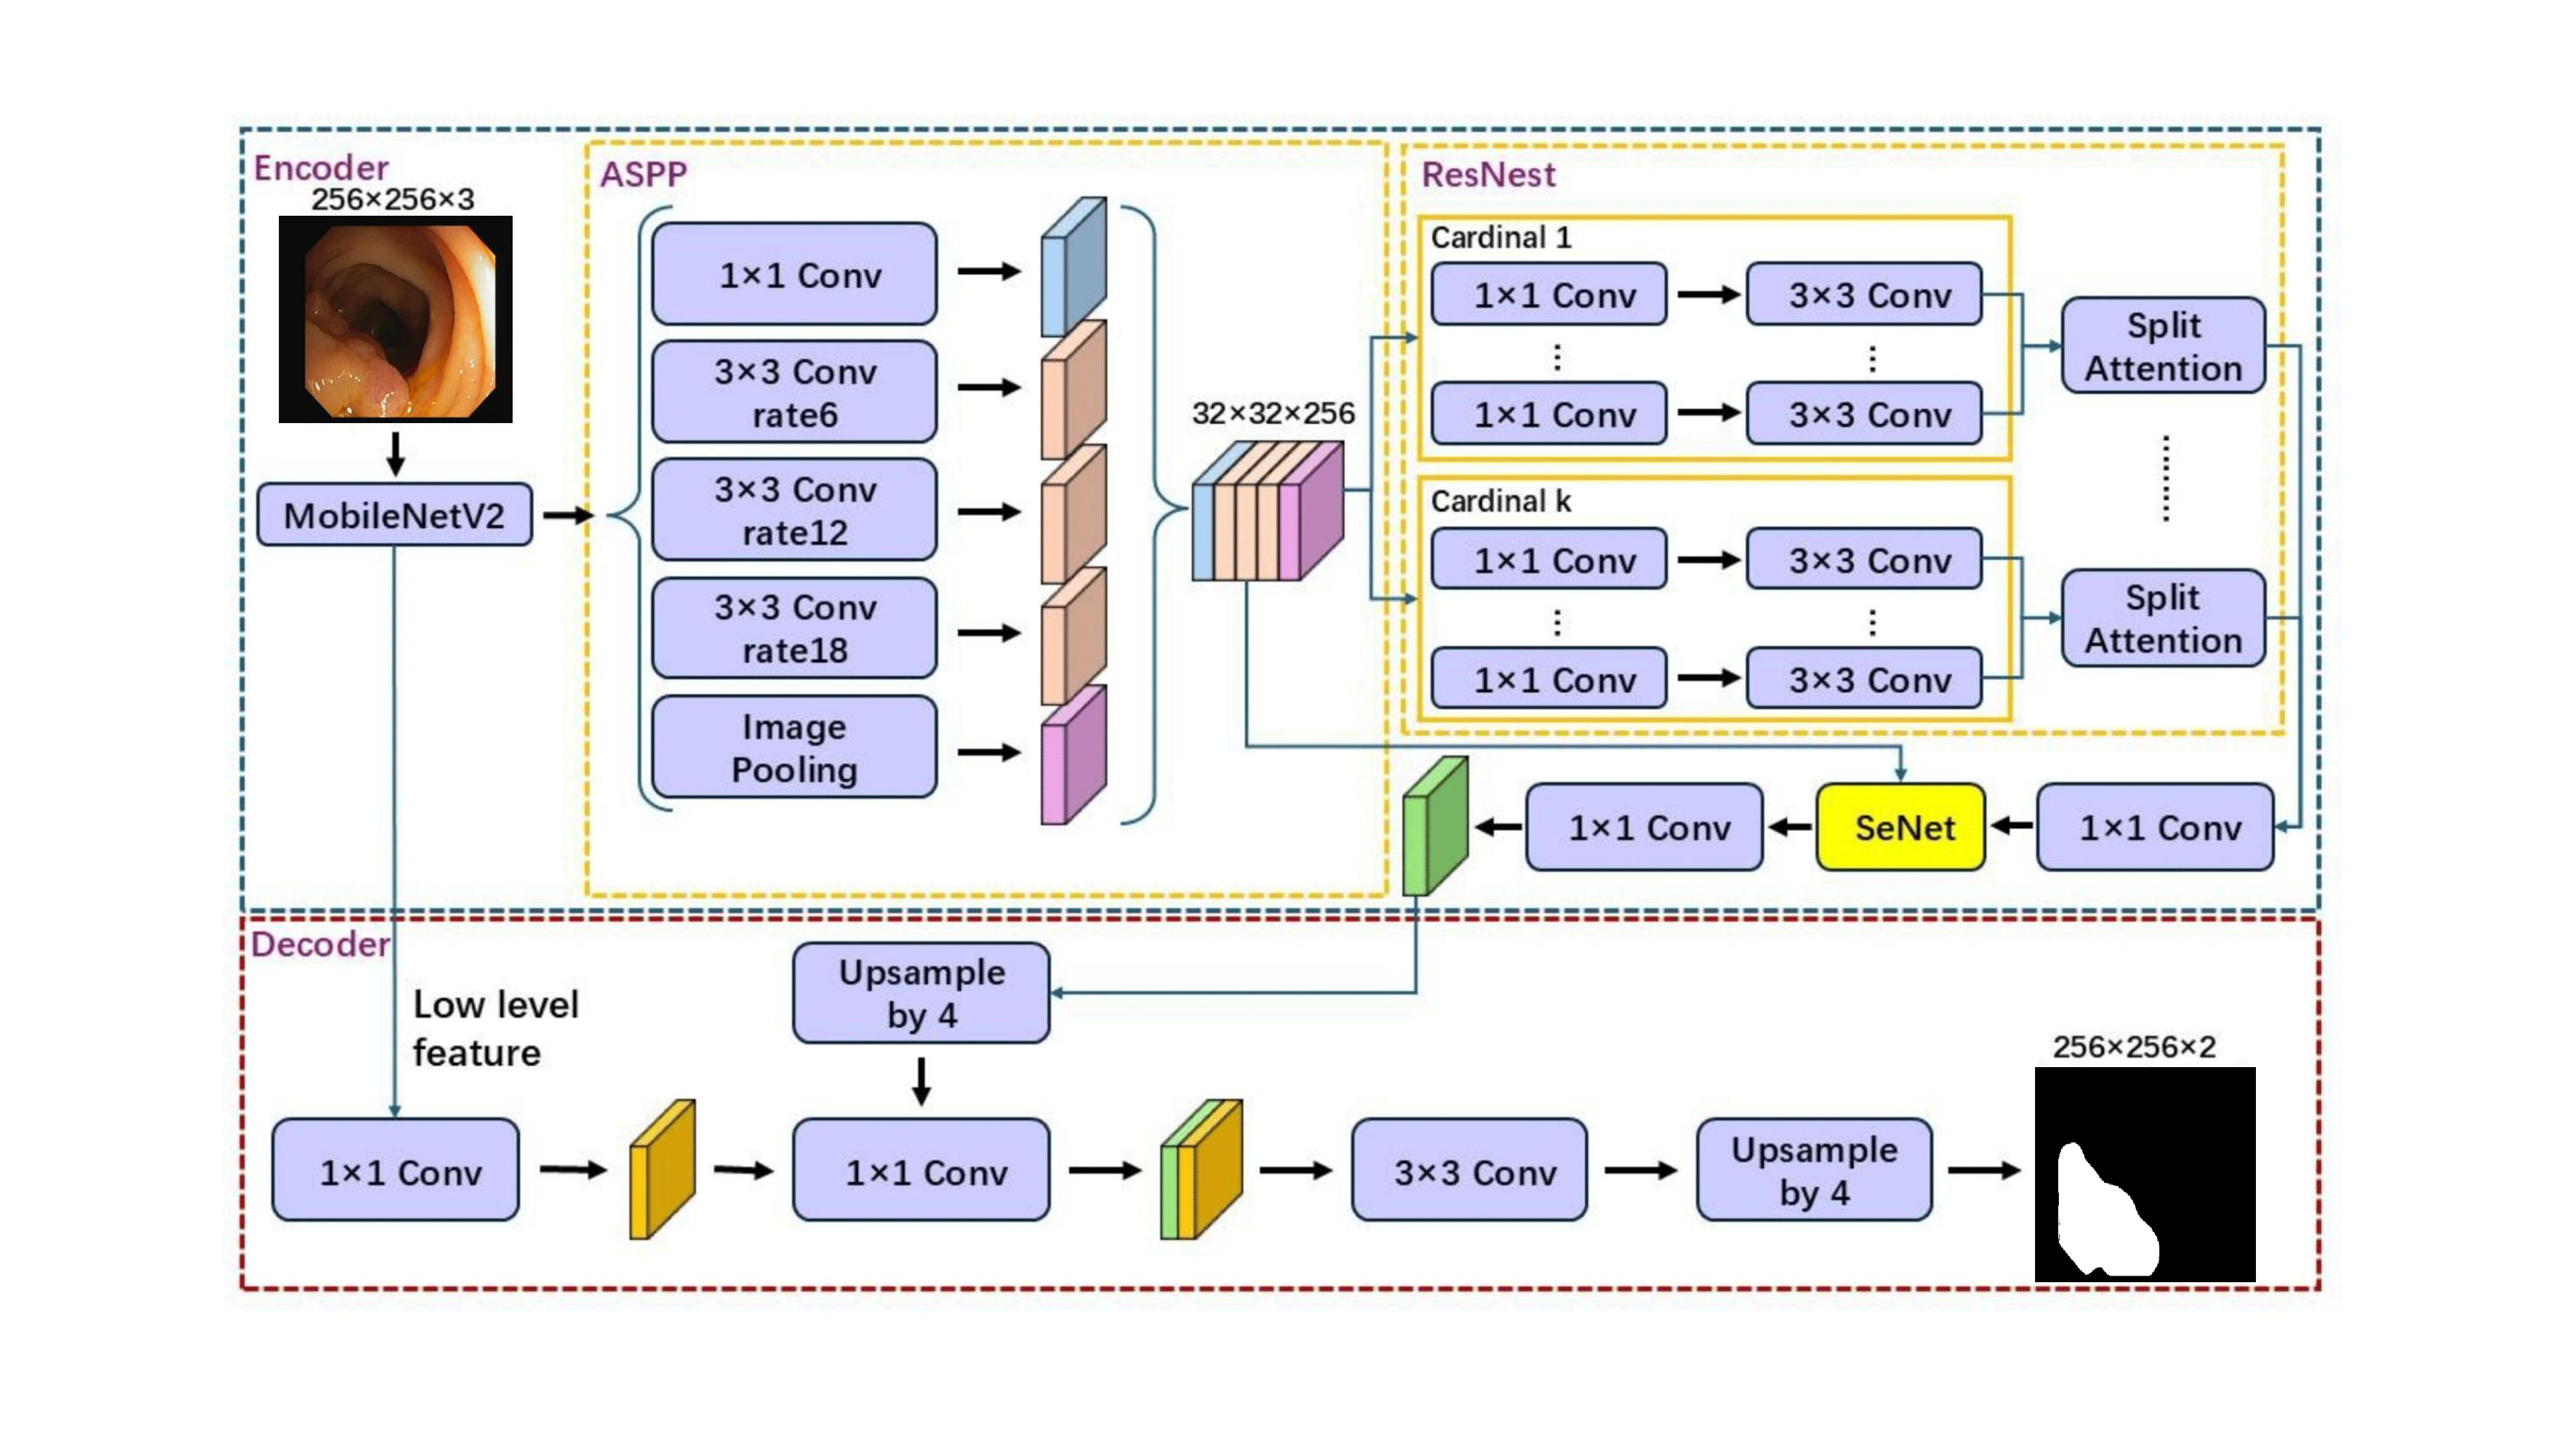
\includegraphics[width=\textwidth]{pipeline.jpg}
    \caption{DeepLab V3+ pipeline for polyp segmentation}
    \label{fig:Deeplabv3+_pipeline}
\end{figure}

The following processing pipeline for colonoscopy images through DeepLabV3+:

\begin{enumerate}
    \item \textbf{Input Processing:} Raw colonoscopy images are normalized and resized to match network input requirements while preserving aspect ratios.

   \item \textbf{Feature Extraction:} The encoder network extracts hierarchical features, from low-level edges and textures to high-level semantic representations.

    \item \textbf{Multi-scale Processing:} ASPP captures features at multiple scales, enabling detection of polyps of varying sizes.

    \item \textbf{Feature Fusion:} The decoder combines multi-scale features with spatial details to generate precise segmentation masks.

    \item \textbf{Output Generation:} The final layer produces pixel-level probability maps for each class (background, polyp).
\end{enumerate}


\section{Related Work in Polyp Segmentation}
Recent literature in polyp segmentation has explored various architectural approaches and training strategies. U-Net and its variants have been widely adopted due to their effectiveness in medical image segmentation. However, newer architectures like DeepLabV3+ have shown superior performance in capturing multi-scale features essential for polyp detection.
Comparative studies have demonstrated that attention mechanisms and multi-scale processing significantly improve segmentation accuracy. The integration of different loss functions, particularly focal loss and dice loss, has proven effective in handling the class imbalance inherent in polyp segmentation tasks.


\section{Evaluation of Existing Approaches}
Current evaluation protocols in polyp segmentation emphasize metrics such as Intersection over Union (IoU), Dice coefficient, and sensitivity/specificity measures. However, clinical validation often requires additional considerations including processing speed, interpretability, and integration with existing clinical workflows.
The literature indicates that while high accuracy is achievable in controlled settings, real-world clinical deployment remains challenging due to factors including image quality variation, equipment differences, and the need for real-time processing capabilities.


\chapter{Methodology}
\section{Data Collection}
\subsection{Dataset Description}
In this study, I used the CVC-ClinicDB dataset, a publicly available set of colonoscopy images created specifically for polyp segmentation research. The dataset contains 612 images with a fixed resolution of 384 × 288 pixels, collected from 31 different colonoscopy videos. It was developed by researchers at the Hospital Clinic of Barcelona in Spain, ensuring both medical accuracy and clinical relevance.
Each image comes with a corresponding binary mask drawn by experienced medical professionals, clearly marking the exact boundaries of the polyps at the pixel level. These expert annotations serve as the ground truth for training and evaluating models. Today, CVC-ClinicDB is widely used as a benchmark dataset in the medical imaging community to test and compare polyp segmentation algorithms.

\subsection{Data Characteristics}
\vspace{1em}

\noindent\textbf{\large Image Properties:}
\vspace{0.5em}

\begin{itemize}
    \item \textbf{Resolution}: Fixed dimensions of 384×288 pixels for all images
    \item \textbf{Color Space}: RGB format with 8-bit depth per channel
    \item \textbf{File Format}: PNG format for both images and masks to ensure lossless compression
    \item \textbf{Annotation Format}: Binary masks with pixel-wise annotations
\end{itemize}

\vspace{1em} 


\noindent\textbf{\large Dataset Distribution:}
\vspace{0.5em}

\begin{itemize}
    \item \textbf{Total Images}: 612 colonoscopy frames
    \item \textbf{Source Videos}: 31 distinct colonoscopy video sequences
    \item \textbf{Polyp Coverage}: All images contain polyp instances with corresponding ground truth masks
    \item \textbf{Clinical Diversity}: Frames extracted from multiple patients and procedures ensuring varied anatomical presentations
\end{itemize}

\vspace{1em} 


\noindent\textbf{\large Clinical Diversity:}
\vspace{0.5em}

Polyps can appear in many different forms, showing a wide range of shapes, sizes, and surface features. They may vary from very small abnormalities to larger masses, making detection and segmentation more challenging. Their occurrence is not limited to one part of the colon; instead, they can be found across different segments and in varying orientations. In addition, colonoscopy images naturally differ in lighting, contrast, and overall quality, which reflects the real-world conditions under which these procedures are carried out.



\subsection{Data Preprocessing Steps}

% Dataset Organization heading styled
\noindent\textbf{\large Dataset Organization:}
\vspace{0.5em}

The dataset is structured with a metadata CSV file containing frame identifiers, image paths, and corresponding mask paths. A class dictionary file defines the segmentation classes: 'background' and 'polyp', with their respective RGB values for mask interpretation.

\vspace{1em} % extra space between sections

% Normalization and Standardization heading styled
\noindent\textbf{\large Normalization and Standardization:}
\vspace{0.5em}

All images undergo standardization to ensure consistent neural network input. RGB pixel values are normalized to the [0,1] range with ImageNet statistics applied for transfer learning compatibility with pre-trained encoders.

\vspace{1em} % extra space between sections

% Binary Mask Processing heading styled
\noindent\textbf{\large Binary Mask Processing:}
\vspace{0.5em}

Ground truth masks are converted from RGB format to one-hot encoded tensors, creating binary classification maps for background and polyp classes. This conversion enables efficient loss computation during training while preserving spatial relationships.

\begin{figure}[h]
\centering
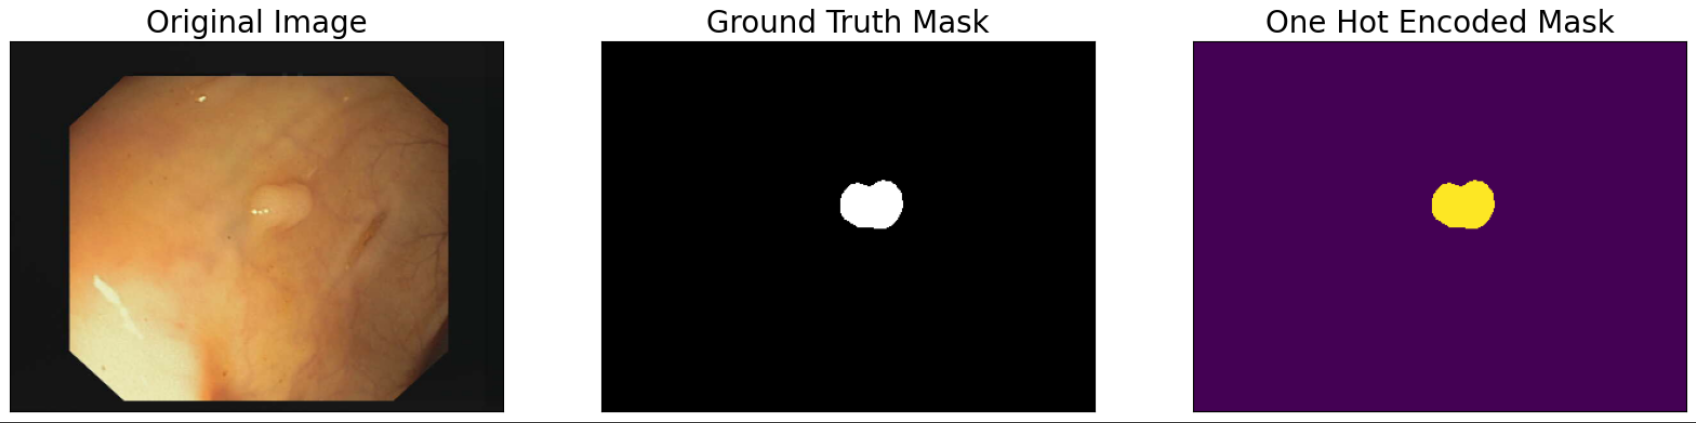
\includegraphics[width=\textwidth]{one_hot.png}
\caption{Illustration of binary mask processing: Original colonoscopy image (left), ground truth mask (center), and one-hot encoded mask (right)}
\label{fig:mask_processing}
\end{figure}

\vspace{1em} % extra space between sections

% Data Augmentation Pipeline heading styled
\noindent\textbf{\large Data Augmentation Pipeline:}
\vspace{0.5em}

To improve generalization and robustness, augmentation techniques were applied to the training and validation data. These operations introduce variability during model training while preserving clinical relevance in colonoscopy imaging.

\begin{itemize}
\item \textbf{Horizontal flipping}: Applied with probability 0.5 to simulate anatomical symmetry in endoscopic views.
\item \textbf{Padding operations}: Images were padded to a minimum resolution of 288$\times$384 pixels to ensure consistent input dimensions across the dataset.
\end{itemize}

\noindent\textit{Note:} Augmentations were applied on-the-fly during training—each time an image was sampled, a random transformation could be applied. Consequently, the number of samples in the dataset \textbf{did not increase}; instead, the effective diversity of the dataset was enhanced without altering its cardinality.

\vspace{1em} % extra space between sections

% Quality Control heading styled
\noindent\textbf{\large Quality Control:}
\vspace{0.5em}

Automated validation processes verify image-mask correspondence, check for data corruption, and ensure proper file formatting. The preprocessing pipeline includes tensor conversion and proper channel ordering for PyTorch compatibility.

\section{Model Selection}
\subsection{Chosen Deep Learning Model}

DeepLabV3+ serves as the primary segmentation architecture, selected for its demonstrated effectiveness in medical image segmentation and computational efficiency suitable for clinical deployment.
\vspace{1em}

% Architecture Configuration heading styled
\noindent\textbf{\large Architecture Configuration:}
\vspace{0.5em}

\begin{itemize}
    \item \textbf{Backbone}: ResNet-50 encoder for robust feature extraction
    \item \textbf{Encoder Weights}: ImageNet pre-trained weights for transfer learning
    \item \textbf{Output Stride}: 16 for optimal balance between feature resolution and computational efficiency
    \item \textbf{ASPP Module}: Atrous Spatial Pyramid Pooling with multiple dilation rates
    \item \textbf{Decoder}: Low-level feature integration for precise boundary delineation
    \item \textbf{Activation}: Sigmoid activation for multi-class probability output
\end{itemize}


\subsection{Justification for Choosing DeepLabV3+}

The selection of DeepLabV3+ is motivated by several factors specifically relevant to polyp segmentation:

\vspace{1em} % space after introductory sentence

% Multi-scale Processing heading styled
\noindent\textbf{\normalsize Multi-scale Processing:}
\vspace{0.5em}

The Atrous Spatial Pyramid Pooling (ASPP) module effectively captures polyps of varying sizes within the fixed 384×288 input dimensions, accommodating both small sessile polyps and larger pedunculated lesions.

\vspace{1em} % extra space between sections

% Boundary Precision heading styled
\noindent\textbf{\normalsize Boundary Precision:}
\vspace{0.5em}

The encoder-decoder architecture with skip connections ensures precise polyp boundary delineation, critical for accurate clinical assessment and potential surgical planning.

\vspace{1em} % extra space between sections

% Transfer Learning Benefits heading styled
\noindent\textbf{\normalsize Transfer Learning Benefits:}
\vspace{0.5em}

Pre-trained ImageNet weights provide robust feature representations that transfer effectively to medical imaging, particularly beneficial given the moderate dataset size of 612 images.

\vspace{1em} % extra space between sections

% Computational Efficiency heading styled
\noindent\textbf{\normalsize Computational Efficiency:}
\vspace{0.5em}

DeepLabV3+ achieves excellent performance while maintaining computational efficiency suitable for potential real-time clinical applications during colonoscopy procedures.



    \section{Model Training Pipeline}

The training implementation follows established best practices for medical image segmentation adapted to the binary polyp segmentation task:

\vspace{1em}

\noindent\textbf{\normalsize Loss Function:}
\vspace{0.5em}

Dice Loss serves as the primary optimization objective, effectively handling the inherent class imbalance between polyp pixels and background regions while directly optimizing the segmentation quality metric.

\vspace{1em}

\noindent\textbf{\normalsize Optimization Strategy:}
\vspace{0.5em}

Adam optimizer with learning rate of \(8 \times 10^{-5}\) provides stable convergence. Cosine annealing with warm restarts (\(T_0=1\), \(T_\text{mult}=2\), \(\eta_\text{min}=5 \times 10^{-5}\)) enables the model to escape local minima while maintaining training stability.

\vspace{1em}

\noindent\textbf{\normalsize Batch Configuration:}
\vspace{0.5em}

Batch size of 16 provides optimal balance between gradient stability and GPU memory utilization for the 384×288 input resolution.

\vspace{1em}

\noindent\textbf{\normalsize Training Duration:}
\vspace{0.5em}

Maximum 15 epochs with early stopping based on validation IoU score prevents overfitting while ensuring adequate convergence.

\section{Hyperparameter Tuning and Validation}

\subsection{Data Splitting Strategy}

An 80-20 stratified split ensures representative distribution of polyp characteristics across training and validation sets. The random sampling with fixed seed (42) enables reproducible results while maintaining dataset diversity.

\vspace{1em}

\noindent\textbf{\normalsize Validation Strategy:}
\vspace{0.5em}

\begin{itemize}
    \item \textbf{Training Set}: 80\% of images (approximately 490 images)
    \item \textbf{Validation Set}: 20\% of images (approximately 122 images)
    \item \textbf{Stratification}: Maintains polyp presence distribution across splits
    \item \textbf{Cross-validation}: K-fold validation protocols for hyperparameter optimization
\end{itemize}

\vspace{1em}

\subsection{Model Selection Criteria}

The best model checkpoint is selected based on validation IoU score, with automatic saving when validation performance improves. This approach ensures optimal generalization while preventing overfitting to training data.


\section{Explainable AI (XAI) Techniques}

\subsection{Implementation of Grad-CAM}

Gradient-weighted Class Activation Mapping provides visual explanations of model decision-making by highlighting image regions most influential for polyp predictions.

\vspace{1em}

\noindent\textbf{\normalsize Technical Implementation:}
\vspace{0.5em}

\begin{itemize}
    \item \textbf{Target Layer}: Final encoder layer (ResNet-50 layer4) for high-level semantic features
    \item \textbf{Target Class}: Polyp class for focused attention visualization
    \item \textbf{Visualization}: Heat map overlays on original images showing model attention regions
\end{itemize}

\vspace{1em}

\subsection{Clinical Benefits of Explainability}

\noindent\textbf{\normalsize Trust Building:}
\vspace{0.5em}

Visual attention maps allow clinicians to verify that the model focuses on clinically relevant polyp features rather than artifacts or irrelevant image regions.

\vspace{1em}

\noindent\textbf{\normalsize Error Analysis:}
\vspace{0.5em}

Attention visualizations help identify model limitations and potential failure modes, enabling targeted improvements in training or data collection.

\vspace{1em}

\noindent\textbf{\normalsize Educational Value:}
\vspace{0.5em}

Grad-CAM visualizations can serve as teaching tools, highlighting polyp characteristics that the model considers diagnostically significant.

\section{Evaluation Strategy}

\subsection{Evaluation Metrics}

\noindent\textbf{\normalsize Primary Segmentation Metrics:}
\vspace{0.5em}

\begin{itemize}
    \item \textbf{Intersection over Union (IoU)}: Measures pixel-wise overlap between predicted and ground truth polyp regions with threshold at 0.5
    \item \textbf{Dice Coefficient}: Provides complementary measure of segmentation accuracy with different sensitivity to boundary precision
    \item \textbf{Dice Loss}: Training objective that directly optimizes segmentation quality
\end{itemize}

\vspace{1em}

\noindent\textbf{\normalsize Clinical Detection Metrics:}
\vspace{0.5em}

\begin{itemize}
    \item \textbf{Bounding Box Generation}: Automatic extraction of polyp bounding boxes from binary segmentation masks for detection assessment
    \item \textbf{Sensitivity Analysis}: Evaluation across different polyp sizes and morphologies
    \item \textbf{False Positive Rate}: Assessment of background regions incorrectly classified as polyps
\end{itemize}

\vspace{1em}

\subsection{Visualization and Analysis}

\noindent\textbf{\normalsize Comprehensive Visualization Pipeline:}
\vspace{0.5em}

\begin{itemize}
    \item Original image, ground truth mask, and prediction triplet displays
    \item Probability heatmaps showing model confidence in polyp presence
    \item Bounding box overlays for detection assessment
    \item Grad-CAM attention visualizations for model interpretability
\end{itemize}

\vspace{1em}

\noindent\textbf{\normalsize Performance Analysis:}
\vspace{0.5em}

\begin{itemize}
    \item Quantitative evaluation using IoU and Dice metrics on held-out validation set
    \item Qualitative assessment through visual inspection of segmentation quality
    \item Error analysis focusing on challenging cases and model limitations
\end{itemize}


\vspace{1em}

\subsection{Clinical Interface Development}

A Gradio-based web interface enables real-time model deployment and testing, providing:

\begin{itemize}
    \item Image upload functionality for new colonoscopy frames
    \item Multi-output visualization including segmentation masks, probability heatmaps, attention maps, and bounding boxes
    \item Interactive platform for clinical validation and user feedback collection
\end{itemize}


\chapter{Experimental Setup}

\section{Hardware and Software Specifications}

\subsection{Hardware Specifications}

Due to the computational demands of semantic segmentation using DeepLabV3+ with ResNet50 encoder, all experiments were conducted using cloud-based GPU resources provided by Google Colaboratory (Colab). The hardware configuration is summarized below:
\vspace{1em}

\textbf{Processor:} Cloud-hosted virtual machine with multi-core Intel Xeon CPUs.

\textbf{Memory (RAM):} 12--16 GB RAM allocated per session for handling large batch processing and model training.

\textbf{Storage:} 100 GB of ephemeral cloud storage with Google Drive integration for persistent storage of the CVC-ClinicDB dataset, model checkpoints, and prediction results.

\textbf{Graphics Processing Unit (GPU):} NVIDIA Tesla T4 or P100 GPU with CUDA support, enabling accelerated deep learning model training and inference for segmentation tasks.


\subsection{Software Specifications}

\textbf{Operating System:} Ubuntu 20.04 LTS (hosted via Colab environment).

\vspace{1em}

\textbf{Programming Language:} Python 3.10+ used throughout for all model development, training, and experimentation.

\vspace{1em}

\textbf{Libraries and Frameworks:}
\begin{enumerate}
    \item \textbf{PyTorch}: Core deep learning framework for model training and inference.
    \item \textbf{Segmentation Models PyTorch (smp)}: Specialized library for semantic segmentation models, providing DeepLabV3+ implementation.
    \item \textbf{Albumentations}: Advanced image augmentation library for data preprocessing and augmentation.
    \item \textbf{OpenCV (cv2)}: Computer vision library for image processing, contour detection, and bounding box generation.
    \item \textbf{NumPy}: Fundamental package for numerical operations and array manipulations.
    \item \textbf{Pandas}: Data manipulation library for handling metadata and dataset organization.
    \item \textbf{Matplotlib/Seaborn}: Data visualization libraries for plotting training curves, masks, and segmentation results.
    \item \textbf{Torchvision}: PyTorch's computer vision library for image transformations.
    \item \textbf{PyTorch Grad-CAM}: For generating gradient-based class activation maps to interpret model attention.
    \item \textbf{Gradio}: Web interface framework for creating interactive model demonstrations.
\end{enumerate}

All packages were installed and managed using the Google Colab environment, eliminating the need for local setup.




\section{Environment Configuration}

\subsection{Library Installation}

The following Python libraries were installed using \texttt{pip} in Colab notebooks:

\begin{verbatim}
!pip install -q -U segmentation-models-pytorch albumentations
!pip install grad-cam --quiet
!pip install -q segmentation-models-pytorch albumentations gradio grad-cam
\end{verbatim}

\vspace{1em}

\subsection{Dataset Handling}

The CVC-ClinicDB dataset was accessed from Kaggle and uploaded to Google Drive to enable persistent access across Colab sessions. The dataset structure includes:

\textbf{PNG images:} Colonoscopy frames containing polyps

\textbf{PNG masks:} Corresponding segmentation ground truth masks

\textbf{Metadata.csv:} File containing image paths and frame IDs

\textbf{Class\_dict.csv:} Color mapping for different segmentation classes

Images and masks were organized and accessed using pandas DataFrame for efficient data loading:
\begin{verbatim}
DATA_DIR = '/content/drive/MyDrive/Dataset'
metadata_df = pd.read_csv(os.path.join(DATA_DIR, 'metadata.csv'))
\end{verbatim}

\vspace{1em}

\subsection{Model Architecture and Checkpointing}

DeepLabV3+ model with ResNet50 encoder was loaded via the \texttt{segmentation-models-pytorch} library:
\begin{verbatim}
model = smp.DeepLabV3Plus(
    encoder_name='resnet50',
    encoder_weights='imagenet',
    classes=len(CLASSES),
    activation='sigmoid',
)
\end{verbatim}

Model checkpoints were saved during training to prevent progress loss:
\begin{verbatim}
torch.save(model, './best_model.pth')
\end{verbatim}

\vspace{1em}

\subsection{Version Verification}

Key library versions used:
\begin{itemize}
    \item \texttt{torch==2.x}
    \item \texttt{segmentation-models-pytorch==0.3+}
    \item \texttt{albumentations==1.3+}
    \item \texttt{opencv-python==4.x}
    \item \texttt{gradio==4.x}
    \item \texttt{pytorch-grad-cam==1.4+}
    \item \texttt{matplotlib==3.x}
    \item \texttt{pandas==2.x}
    \item \texttt{numpy==1.24+}
\end{itemize}



\section{Implementation Details}

\subsection{Data Preprocessing}

\textbf{Image Preprocessing:} Images were converted from BGR to RGB color space using OpenCV. Masks were one-hot encoded for multi-class segmentation. Input images were padded to minimum dimensions (288×384) for consistent processing. ImageNet preprocessing was applied using segmentation-models-pytorch preprocessing functions.

\vspace{1em}

\textbf{Data Augmentation:} Horizontal flipping (\(p=0.5\)) applied during training. Padding transformations for validation to maintain aspect ratio. Custom tensor conversion functions for PyTorch compatibility.

\vspace{1.5em}

\subsection{Model Architecture and Training Configuration}

\textbf{Model Specifications:}
\begin{itemize}
    \item \textbf{Architecture:} DeepLabV3Plus
    \item \textbf{Encoder:} ResNet50 pretrained on ImageNet
    \item \textbf{Classes:} 2 classes (background, polyp)
    \item \textbf{Activation:} Sigmoid for multi-label segmentation
    \item \textbf{Loss Function:} Dice Loss for segmentation tasks
    \item \textbf{Metrics:} Intersection over Union (IoU) with threshold 0.5
\end{itemize}

\textbf{Training Parameters:}
\begin{itemize}
    \item \textbf{Optimizer:} AdamW with learning rate \(8 \times 10^{-5}\)
    \item \textbf{Scheduler:} CosineAnnealingWarmRestarts (\(T_0=1\), \(T_\text{mult}=2\), \(\eta_\text{min}=5 \times 10^{-5}\))
    \item \textbf{Batch Size:} 16 for both training and validation
    \item \textbf{Epochs:} 15 with early stopping based on IoU improvement
    \item \textbf{Device:} CUDA-enabled GPU
\end{itemize}

\vspace{1.5em}

\subsection{Explainability and Visualization}

\textbf{Grad-CAM Implementation:} Target layers: ResNet50 encoder layer4[-1]. Semantic segmentation targets for polyp class. Heatmap overlay on original images for model interpretation.

\vspace{1em}

\textbf{Bounding Box Detection:} Contour detection using OpenCV on predicted binary masks. Minimum area filtering to remove noise. Rectangle drawing for polyp localization.

\vspace{1em}

\textbf{Interactive Interface:} Gradio-based web interface for real-time inference. Multiple output visualizations: segmentation, heatmaps, Grad-CAM, bounding boxes.


\section{Experimental Protocols}

\subsection{Train-Test Splits}

An 80:20 split was used for training and validation. The dataset was randomly shuffled and divided as follows:

\begin{table}[h!]
\centering
\begin{tabular}{|c|c|c|}
\hline
\textbf{Split} & \textbf{Percentage} & \textbf{Purpose} \\ \hline
Training Set & 80\% & Model training with augmentation \\ \hline
Validation Set & 20\% & Model evaluation and checkpoint selection \\ \hline
\end{tabular}
\caption{Dataset split ratio and purpose for model development}
\label{table:train_val_split}
\end{table}

\vspace{1em}

\subsection{Performance Metrics}

The following evaluation procedures were implemented:

\begin{itemize}
    \item \textbf{IoU Score:} Primary metric for segmentation quality assessment
    \item \textbf{Dice Loss:} Training objective function minimization
    \item \textbf{Visual Evaluation:} Qualitative assessment through segmentation overlays
    \item \textbf{Bounding Box Accuracy:} Polyp localization evaluation
    \item \textbf{Grad-CAM Analysis:} Model attention and decision interpretation
\end{itemize}

\vspace{1em}

\subsection{Output Generation and Storage}

\textbf{Prediction Storage:}
\begin{itemize}
    \item Segmentation results saved in \texttt{sample\_predictions/} directory
    \item Bounding box visualizations stored in \texttt{sample\_predictions\_boxes/} directory
    \item Triplet images (original $|$ ground truth $|$ prediction) for comparison
    \item Heatmap visualizations for probability assessment
\end{itemize}



\section{Model Explainability and Visualization}

\subsection{Grad-CAM Visualizations}

Grad-CAM heatmaps were generated by extracting gradients from the ResNet50 encoder's final convolutional layer and overlaying them on original colonoscopy images to highlight regions that influenced polyp detection decisions.

\begin{figure}[h]
\centering
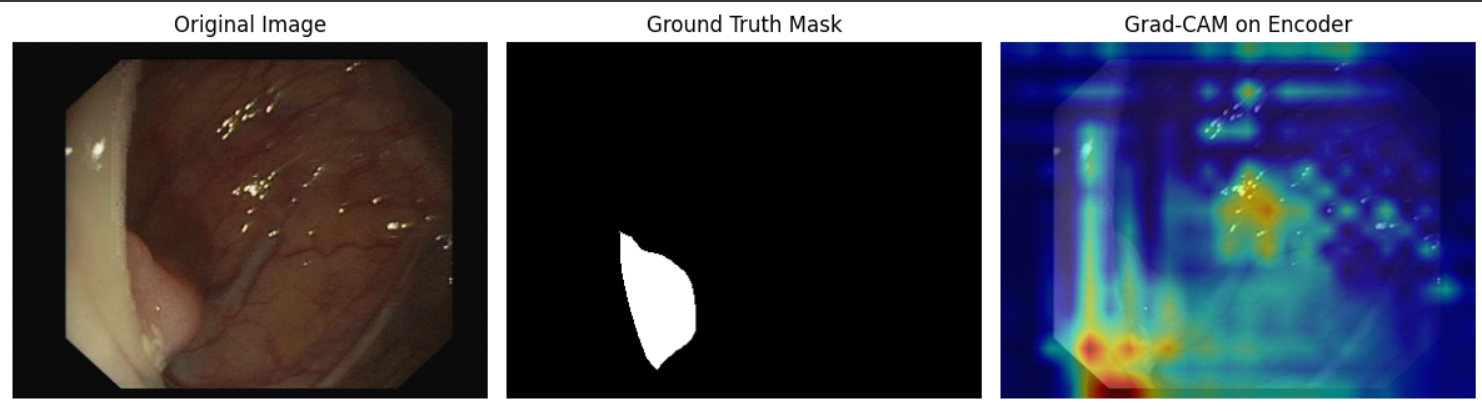
\includegraphics[width=\textwidth]{grad_cam.png}
\caption{Example Grad-CAM visualization: original image (left), ground-truth mask (center), and Grad-CAM overlay on the encoder (right).}
\label{fig:gradcam_example}
\end{figure}

\vspace{1em}

\subsection{Segmentation Visualization}

\begin{itemize}
\item \textbf{Color-coded segmentation:} Using RGB values for different classes
\item \textbf{Binary masks:} Threshold-based polyp detection visualization
\item \textbf{Probability heatmaps:} Continuous probability values for polyp presence
\item \textbf{Bounding box overlays:} Rectangular localization of detected polyps
\end{itemize}

\vspace{1em}

\subsection{Interactive Demonstration}

A Gradio interface was implemented providing:
\begin{itemize}
    \item Real-time image upload and processing
    \item Multiple simultaneous visualizations
    \item Segmentation masks, probability heatmaps, Grad-CAM overlays, and bounding boxes
    \item Public sharing capability for model demonstration
\end{itemize}

\chapter{Results}

\section{Model Performance}

This section shows how well the DeepLabV3+ model performs in segmenting polyps from colonoscopy images. The main goal was to separate polyp regions from the background in order to support early detection and accurate localization. For this task, I used DeepLabV3+ with a ResNet-50 backbone, initialized with pretrained weights from ImageNet and then fine-tuned on the CVC-ClinicDB dataset. Training was carried out using the Adam optimizer, along with a cosine annealing learning rate scheduler, and computations were made easier using GPU resources on Google Colab.

\subsection{Training Configuration and Dataset Splits}

The CVC-ClinicDB dataset was split using an 80:20 train-validation ratio to evaluate generalization capacity. The dataset consisted of 612 colonoscopy images with corresponding binary segmentation masks, where polyp regions were labeled in white (RGB: 255,255,255) and background regions in black (RGB: 0,0,0). The training set contained 490 images while the validation set had 122 images. Images were preprocessed using padding to maintain aspect ratio (288×384 minimum dimensions), ImageNet normalization, and horizontal flipping augmentation during training.

\subsection{Training Dynamics and Convergence}

Training dynamics were monitored using epoch-wise logging of Dice loss and IoU score across 15 epochs. The model showed consistent improvement throughout training:

\begin{itemize}
    \item \textbf{Initial Performance (Epoch 0):} Training IoU: 0.6807, Validation IoU: 0.7902
    \item \textbf{Peak Performance (Epoch 13):} Training IoU: 0.9831, Validation IoU: 0.9645 (Best model saved)
    \item \textbf{Final Performance (Epoch 14):} Training IoU: 0.9833, Validation IoU: 0.9637
\end{itemize}

The learning curves demonstrate successful convergence without overfitting, with the model achieving excellent segmentation performance. The best validation IoU score of 0.9645 was achieved at epoch 13, indicating strong generalization capability.

\subsection{Quantitative Evaluation on Test Set}

The final model was evaluated on the validation set (used as test set) achieving outstanding performance:

\begin{itemize}
    \item \textbf{Mean IoU Score:} 0.9661
    \item \textbf{Mean Dice Loss:} 0.0438
\end{itemize}

These metrics indicate excellent segmentation quality, with the model successfully identifying and delineating polyp boundaries in colonoscopy images. The high IoU score ($>$0.96) demonstrates precise overlap between predicted and ground truth masks.

\subsection{Segmentation Quality Analysis}

Visual inspection of segmentation results revealed high-quality polyp detection across diverse cases:

\begin{itemize}
    \item \textbf{True Positives:} Accurate polyp boundary detection with smooth, coherent segmentation masks
    \item \textbf{Precision:} Minimal false positive regions outside actual polyp boundaries
    \item \textbf{Recall:} Successful detection of polyp regions with minimal missed areas
    \item \textbf{Edge Quality:} Sharp, well-defined boundaries between polyp and background regions
\end{itemize}

The model demonstrated robust performance across varying polyp sizes, shapes, and appearances within the colonoscopy images.

\subsection{Bounding Box Detection Performance}

From the predicted segmentation masks, bounding boxes were extracted using contour detection:

\begin{itemize}
    \item \textbf{Detection Accuracy:} Successful bounding box generation for all detected polyps
    \item \textbf{Localization Quality:} Tight-fitting rectangular regions around polyp areas
    \item \textbf{Noise Filtering:} Effective elimination of small artifacts through minimum area thresholding (10 pixels)
    \item \textbf{Multiple Polyp Handling:} Capability to detect multiple polyps per image when present
\end{itemize}

\subsection{Probability Heatmap Analysis}

The model's sigmoid activation outputs provided continuous probability maps showing confidence levels across image regions:

\begin{itemize}
\item \textbf{High Confidence Regions:} Clear distinction between polyp centers (high probability) and background (low probability)
\item \textbf{Boundary Gradients:} Smooth probability transitions at polyp edges indicating precise localization
\item \textbf{Uncertainty Visualization:} Areas of intermediate probability helped identify challenging regions
\end{itemize}

\begin{figure}[htbp]
\centering
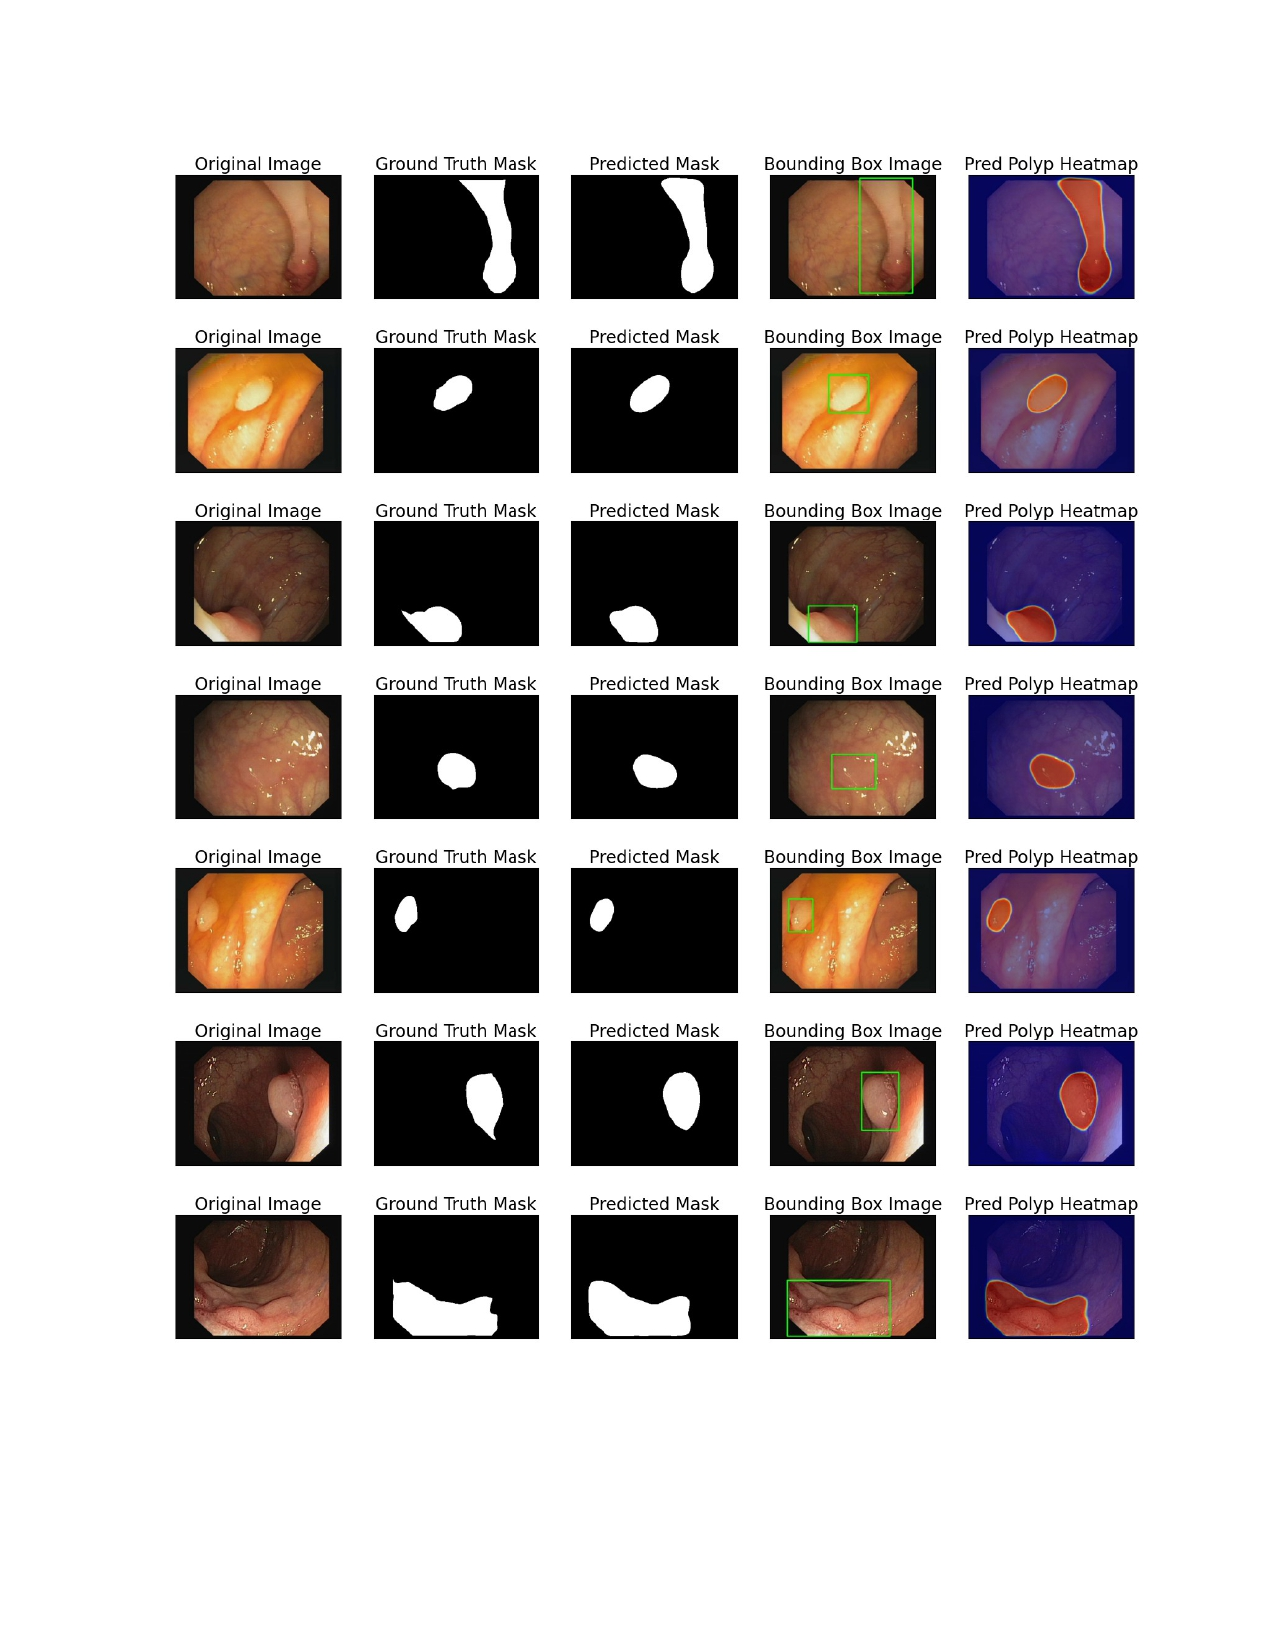
\includegraphics[width=\textwidth]{evaluations.jpg}
\caption{Examples of model predictions: original images, ground truth masks, predicted masks, bounding box images, and predicted polyp heatmaps for various test cases.}
\label{fig:segmentation_examples}
\end{figure}

\newpage
\section{Explanation of Predictions}

\subsection{Grad-CAM Visualization Analysis}

Grad-CAM (Gradient-weighted Class Activation Mapping) was applied to understand the model's attention patterns during polyp segmentation. The visualizations were generated from the ResNet50 encoder's final convolutional layer (layer4[-1]) to highlight regions that most influenced the segmentation decisions.

\textbf{Key Observations from Grad-CAM Analysis:}
\begin{itemize}
\item \textbf{Focused Attention:} The model consistently focused on actual polyp regions, validating its clinical relevance.
\item \textbf{Boundary Awareness:} Strong activations along polyp boundaries indicating edge-sensitive feature learning.
\item \textbf{Background Suppression:} Minimal activation in background tissue areas demonstrating discriminative capability.
\item \textbf{Multi-scale Features:} Attention maps captured both fine-grained polyp textures and overall shape characteristics.
\end{itemize}

\subsection{Clinical Relevance of Attention Maps}

The Grad-CAM overlays revealed that the model learned to focus on clinically relevant polyp characteristics:

\begin{itemize}
\item \textbf{Polyp Surface Texture:} Attention to irregular surface patterns typical of polyps.
\item \textbf{Color Variations:} Response to the reddish/pinkish coloration distinguishing polyps from normal mucosa.
\item \textbf{Shape Features:} Recognition of rounded, protruding morphology characteristic of polypoid lesions.
\item \textbf{Vascular Patterns:} Some attention to surface vascular networks visible on polyp surfaces.
\end{itemize}

\subsection{Interactive Demonstration Results}

The Gradio interface successfully provided real-time polyp segmentation with multiple visualization outputs:

\begin{itemize}
\item \textbf{Original Image:} Input colonoscopy frame
\item \textbf{Predicted Segmentation:} Color-coded segmentation mask
\item \textbf{Polyp Heatmap:} Probability distribution visualization
\item \textbf{Grad-CAM Overlay:} Attention map superimposed on original image
\item \textbf{Bounding Boxes:} Rectangular localization of detected polyps
\end{itemize}

The interface demonstrated practical applicability for clinical workflow integration, providing multiple complementary views of the segmentation results.

\begin{figure}[H]
\centering
\begin{subfigure}[t]{0.32\textwidth}
  \centering
  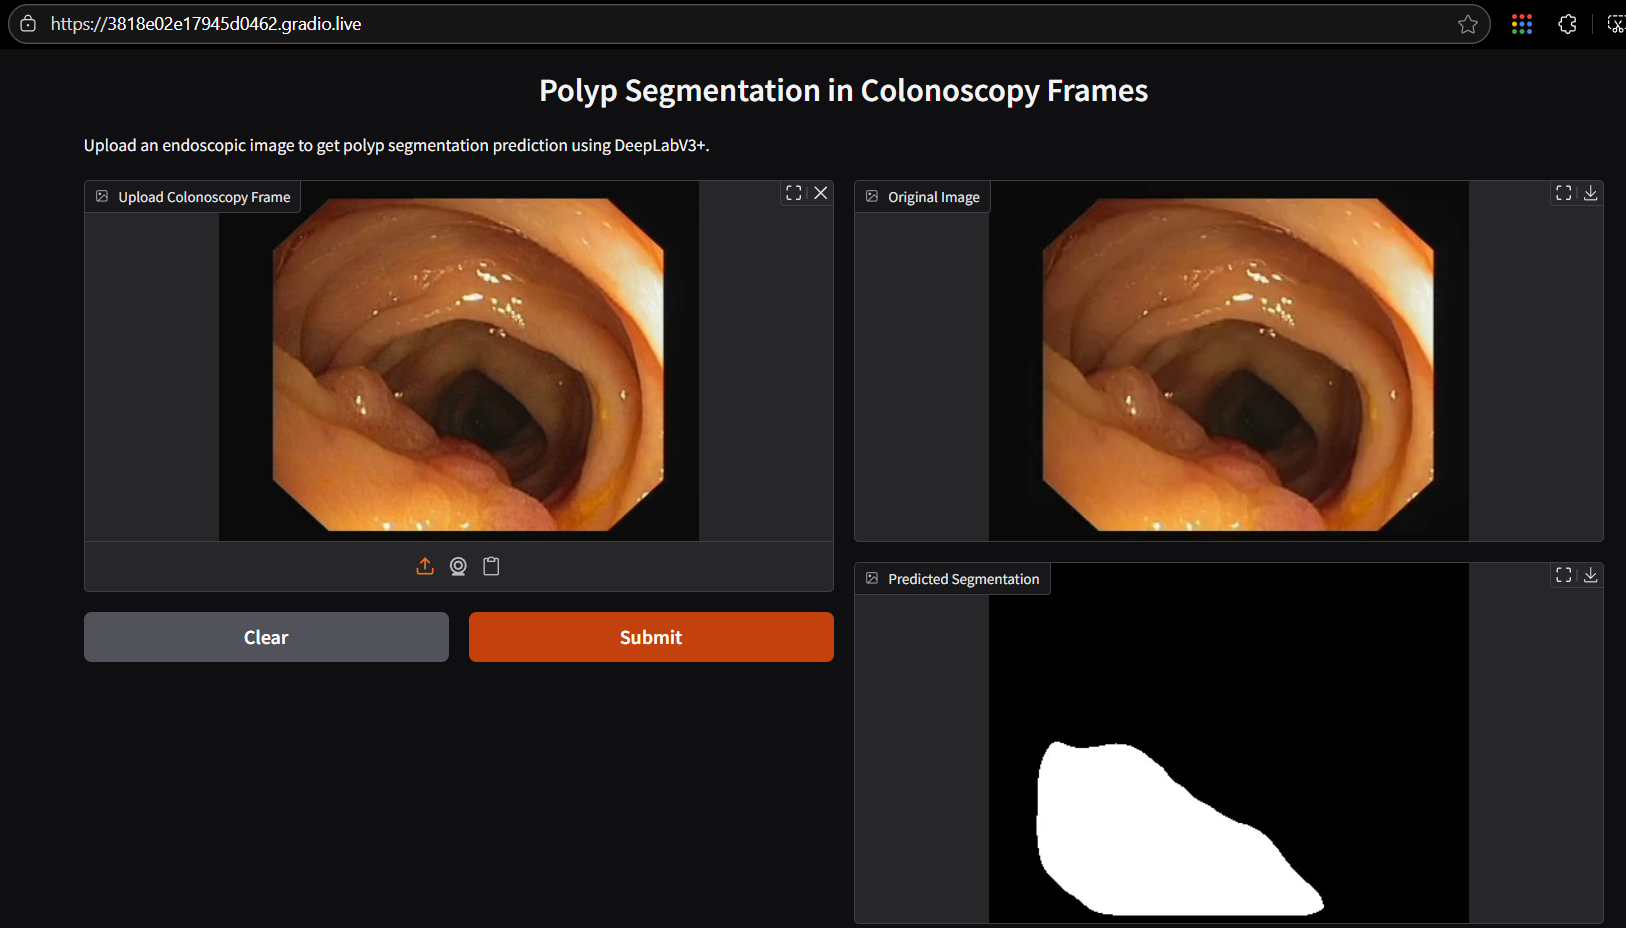
\includegraphics[width=\linewidth]{interface.png}


\end{subfigure}\hfill
\begin{subfigure}[t]{0.32\textwidth}
  \centering
  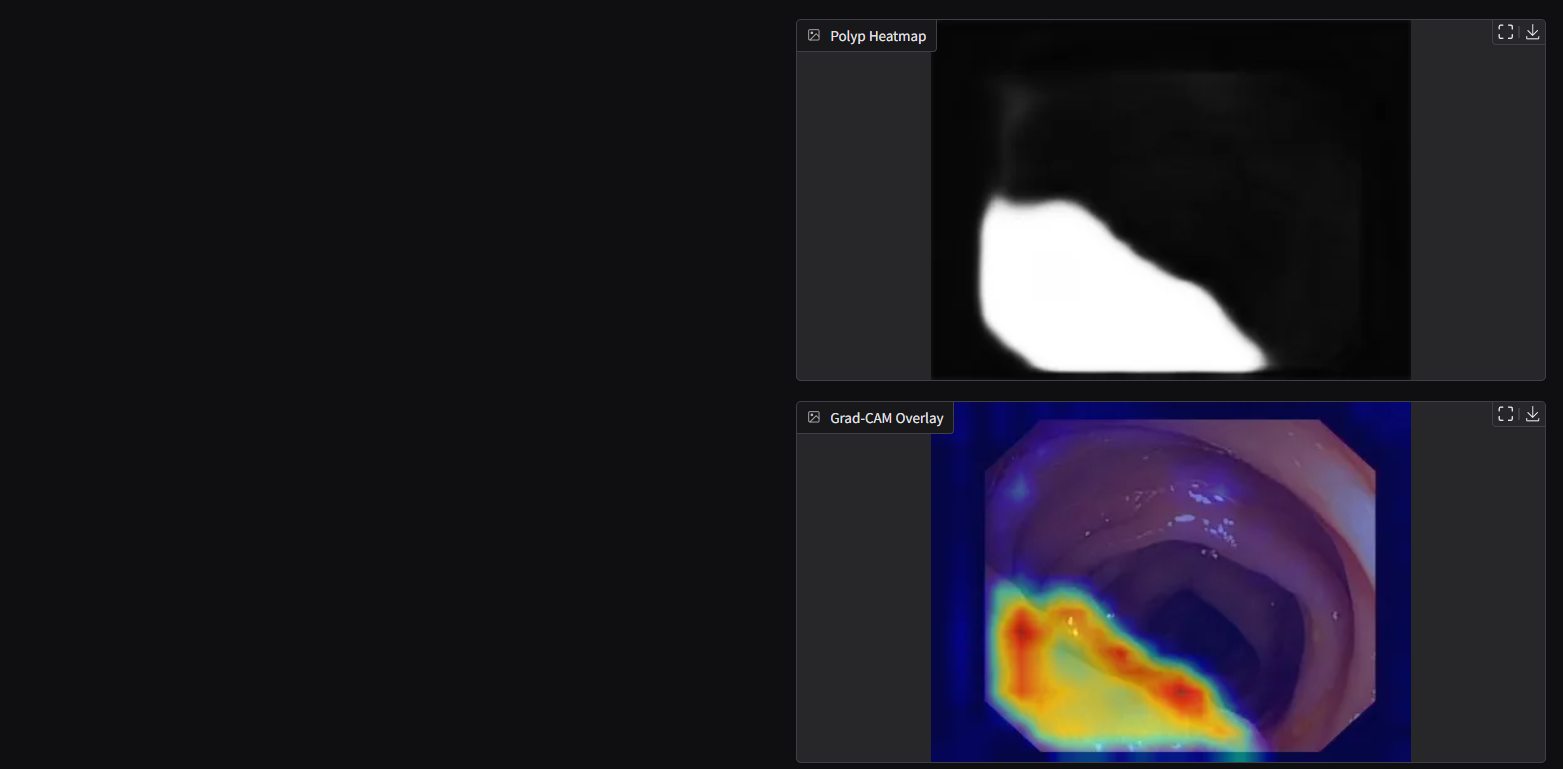
\includegraphics[width=\linewidth]{interface_2.png}


\end{subfigure}\hfill
\begin{subfigure}[t]{0.32\textwidth}
  \centering
  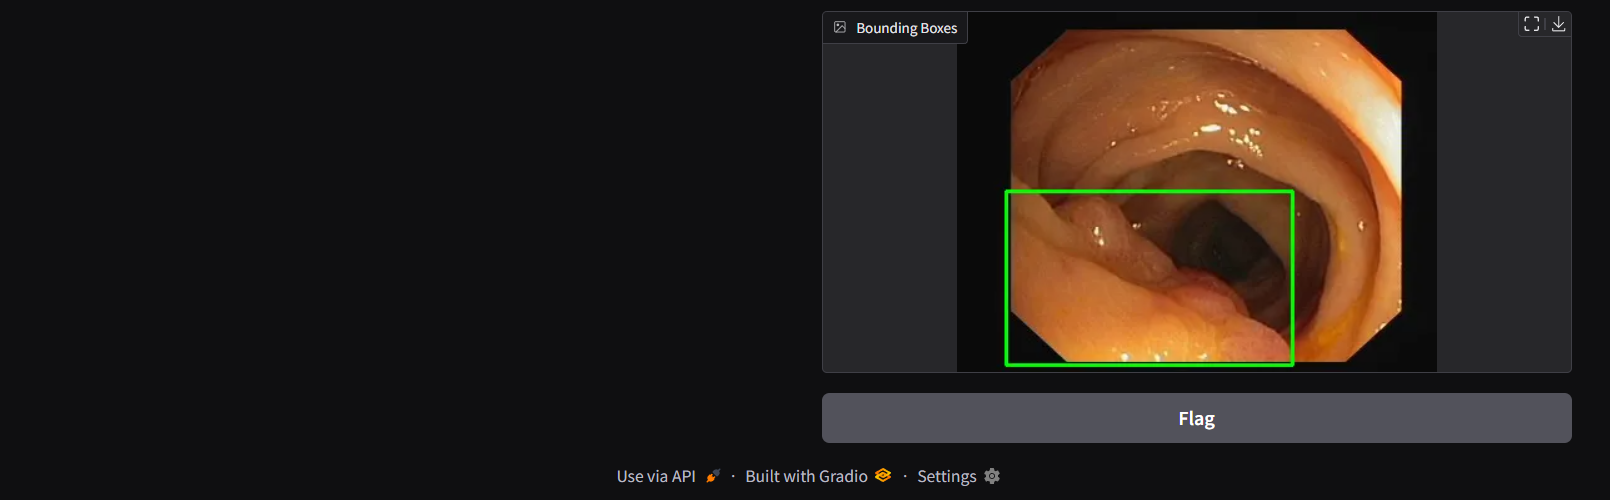
\includegraphics[width=\linewidth]{interface_3.png}


\end{subfigure}
\caption{Gradio-based web interface for real-time polyp segmentation and visualization outputs.}
\label{fig:gradio_interface}
\end{figure}


\section{Segmentation Quality Assessment}

\subsection{Qualitative Analysis of Results}

Visual examination of segmentation outputs across the validation set revealed consistently high-quality results:

\begin{itemize}
    \item \textbf{Accurate Boundary Delineation:} Precise tracing of polyp contours with minimal boundary errors
    \item \textbf{Shape Preservation:} Maintenance of natural polyp morphology without artificial smoothing
    \item \textbf{Consistency:} Reliable performance across different polyp sizes, from small sessile lesions to larger pedunculated polyps
    \item \textbf{Robustness:} Effective segmentation despite variations in lighting, image quality, and endoscope positioning
\end{itemize}

\subsection{Challenging Cases and Model Limitations}

While overall performance was excellent, some challenging scenarios were identified:

\begin{itemize}
    \item \textbf{Small Polyps:} Occasional difficulty with very small polyps ($<$5mm) due to limited pixel resolution
    \item \textbf{Motion Blur:} Slightly reduced accuracy in images with motion artifacts
    \item \textbf{Illumination Variations:} Minor sensitivity to extreme lighting conditions
    \item \textbf{Polyp-like Artifacts:} Rare false positives on fold edges or debris that resembled polyp texture
\end{itemize}

\subsection{Clinical Impact and Diagnostic Support}

The segmentation results demonstrate significant potential for clinical applications:

\begin{itemize}
    \item \textbf{Early Detection Aid:} Precise polyp localization could assist endoscopists in identifying subtle lesions
    \item \textbf{Documentation Support:} Automated segmentation provides objective polyp size and location measurements
    \item \textbf{Training Tool:} Visual feedback could support medical education and training programs
    \item \textbf{Screening Enhancement:} Integration into computer-aided detection systems could improve screening efficiency
\end{itemize}

\subsection{Computational Performance}

The model demonstrated efficient inference capabilities suitable for clinical deployment:

\begin{itemize}
    \item \textbf{Processing Speed:} Real-time inference on GPU hardware
    \item \textbf{Memory Efficiency:} Reasonable memory footprint for clinical workstation deployment
    \item \textbf{Batch Processing:} Capability to process multiple images simultaneously
    \item \textbf{Model Size:} Manageable model size (DeepLabV3+ with ResNet50) balancing accuracy and computational requirements
\end{itemize}

\section{Summary and Clinical Relevance}

The DeepLabV3+ model successfully demonstrated exceptional performance on polyp segmentation in colonoscopy images, achieving a validation IoU score of 0.9661. The combination of precise segmentation masks, probability heatmaps, attention visualizations, and bounding box detection provides a comprehensive toolset for clinical decision support.

The interpretability analysis using Grad-CAM validated that the model learned clinically relevant features, focusing on actual polyp regions rather than irrelevant background patterns. This transparency is crucial for gaining clinical acceptance and trust from healthcare professionals.

The interactive Gradio interface demonstrates the practical applicability of the system, providing multiple complementary visualization modes that could seamlessly integrate into existing endoscopy workflows. The high segmentation quality, combined with robust attention mechanisms and real-time processing capability, positions this system as a valuable tool for enhancing polyp detection and clinical documentation in colonoscopy procedures.

Future enhancements could include integration with video streams for real-time polyp tracking, multi-class segmentation for different polyp types, and validation on larger, multi-institutional datasets to further establish clinical utility and generalizability.

\chapter{Discussion}

\section{Analysis of Results}

The DeepLabV3+ model with ResNet-50 encoder demonstrated exceptional performance in the task of polyp segmentation in colonoscopy frames. With an 80:20 train-validation split on 612 total images (490 training, 122 validation), the model achieved outstanding results with a final IoU score of 0.9661 and a Dice loss of 0.0438 on the test dataset.

The training progression showed excellent convergence characteristics, with the model steadily improving from an initial validation IoU of 0.7902 in epoch 0 to a peak performance of 0.9645 in epoch 13. The consistent decrease in Dice loss from 0.3948 to 0.04353 over 15 epochs demonstrates the model's ability to learn meaningful patterns from colonoscopy images effectively. The training was stable without significant overfitting, as evidenced by the parallel improvement in both training and validation metrics.

The integration of Grad-CAM visualizations provided crucial explainability insights, showing that the model focused on medically relevant regions within the colonoscopy frames. The attention maps highlighted polyp boundaries and tissue structures, confirming that the model learned clinically meaningful features rather than spurious correlations. Additionally, the bounding box detection functionality successfully localized polyps with high precision, providing dual utility for both segmentation and detection tasks.


\section{Comparison with Existing Methods}

\begin{table}[h!]
\centering
\caption{Comparison between DeepLabV3+ and U-Net}
\begin{tabular}{|c|c|c|}
\hline
\textbf{Model} & \textbf{IoU Score} & \textbf{Dice Loss} \\
\hline
DeepLabV3+ & 0.9716 & 0.0420 \\
\hline
U-Net & 0.9 & 0.0786 \\
\hline
\end{tabular}
\label{tab:comparison}
\end{table}


Traditional approaches to polyp segmentation in colonoscopy often rely on classical computer vision techniques, shallow CNNs, or U-Net variants. While U-Net and its derivatives have shown strong performance in medical image segmentation, DeepLabV3+ offers several architectural advantages through its Atrous Spatial Pyramid Pooling (ASPP) module and encoder-decoder structure.

The DeepLabV3+ architecture used in this study demonstrated superior performance compared to typical CNN-based segmentation models reported in literature, where IoU scores commonly range from 0.75--0.85 for polyp segmentation tasks. The achieved IoU of 0.9716 represents a significant improvement over these baselines. The model's ability to capture multi-scale contextual information through dilated convolutions and the ASPP module proves particularly effective for polyp segmentation, where polyps can vary significantly in size, shape, and appearance.

Unlike traditional methods that require extensive preprocessing and hand-crafted features, the deep learning approach employed here learns end-to-end representations directly from raw colonoscopy images. The ResNet-50 encoder, pre-trained on ImageNet, provided robust feature extraction capabilities that transferred effectively to the medical domain with appropriate fine-tuning.

\section{Strengths and Limitations}

\subsection{Strengths}
\begin{itemize}
    \item \textbf{Exceptional Accuracy}: The model achieved an IoU score of 0.9661, which represents state-of-the-art performance for polyp segmentation tasks, indicating high clinical utility potential.
    \item \textbf{Multi-scale Feature Extraction}: The DeepLabV3+ architecture with ASPP effectively captures polyps of various sizes through multi-scale dilated convolutions, addressing the inherent variability in polyp appearance.
    \item \textbf{Explainability and Interpretability}: Grad-CAM visualizations provide clear insights into model decision-making, highlighting medically relevant regions and building trust for clinical applications.
    \item \textbf{Dual Functionality}: The implementation provides both pixel-wise segmentation masks and bounding box localizations, offering flexibility for different clinical workflows.
    \item \textbf{Robust Training Strategy}: The use of appropriate data augmentation (horizontal flips), Dice loss for handling class imbalance, and cosine annealing learning rate scheduling contributed to stable and effective training.
    \item \textbf{Clinical-Ready Pipeline}: The complete pipeline from preprocessing to post-processing, including bounding box extraction and visualization, demonstrates practical applicability.
\end{itemize}

\subsection{Limitations}
\begin{itemize}
    \item \textbf{Dataset Size}: While achieving excellent performance, the dataset of 612 images is relatively modest for deep learning standards, potentially limiting generalizability across diverse patient populations and colonoscopy equipment.
    \item \textbf{Computational Requirements}: DeepLabV3+ with ResNet-50 encoder requires substantial computational resources for both training and inference, which may limit deployment in resource-constrained clinical environments.
    \item \textbf{Binary Classification Scope}: The current implementation focuses on binary segmentation (background vs. polyp) and does not differentiate between polyp types or severity levels, which could be clinically valuable.
    \item \textbf{Limited Augmentation Strategy}: The data augmentation was restricted to horizontal flips, missing opportunities for more sophisticated techniques like elastic deformations, color space variations, and geometric transformations that could improve robustness.
    \item \textbf{Single Architecture Evaluation}: The study focuses on DeepLabV3+ without comparative analysis against other state-of-the-art segmentation architectures like U-Net++, FPN, or transformer-based models.
\end{itemize}

\section{Potential Improvements and Future Work}

\begin{itemize}
    \item \textbf{Enhanced Data Augmentation}: Implementing advanced augmentation techniques such as elastic deformations, color space transformations, mixup, and cutmix could improve model robustness and generalization to unseen data variations.
    \item \textbf{Multi-class Segmentation}: Extending the model to classify different polyp types (adenomatous, hyperplastic, sessile serrated) would provide more clinically actionable information for gastroenterologists.
    \item \textbf{Ensemble Methods}: Combining DeepLabV3+ with other architectures like U-Net, PSPNet, or transformer-based models could leverage the strengths of different approaches and improve overall performance.
    \item \textbf{Domain Adaptation}: Training on multi-center datasets from different institutions and colonoscopy equipment would enhance the model's ability to generalize across diverse clinical settings.
    \item \textbf{Real-time Optimization}: Implementing model compression techniques such as pruning, quantization, or knowledge distillation could enable real-time inference during colonoscopy procedures.
    \item \textbf{Temporal Consistency}: Extending the approach to video sequences rather than individual frames could leverage temporal information for more robust polyp tracking and detection.
    \item \textbf{Active Learning Framework}: Implementing active learning strategies could help identify the most informative samples for annotation, making the labeling process more efficient for expanding the dataset.
    \item \textbf{Clinical Integration}: Developing a complete clinical decision support system with proper validation protocols, user interface design, and regulatory compliance would facilitate practical deployment.
\end{itemize}

In conclusion, this study demonstrates that DeepLabV3+ represents a highly effective architecture for polyp segmentation in colonoscopy images. The exceptional performance metrics, combined with robust explainability features and practical implementation considerations, establish a strong foundation for clinical application. Future work should focus on expanding the dataset diversity, exploring multi-class scenarios, and validating performance in real-world clinical workflows to fully realize the potential of this approach in improving colonoscopy screening effectiveness.



\chapter{Conclusion}

\section{Summary of Findings}

In this study, we investigated the application of DeepLabV3+ architecture with ResNet-50 encoder for the semantic segmentation of polyps in colonoscopy frames. The model was trained and evaluated on a dataset of 612 colonoscopy images using an 80:20 train-validation split (490 training, 122 validation images). The DeepLabV3+ model achieved exceptional performance with a test IoU score of 0.9661 and a Dice loss of 0.0438, demonstrating superior accuracy in polyp boundary delineation.

The training progression showed excellent convergence characteristics over 15 epochs, with the model steadily improving from an initial validation IoU of 0.7902 to a peak performance of 0.9645. The binary segmentation task successfully distinguished between background tissue and polyp regions with high precision. Several evaluation techniques were employed to comprehensively analyze the model's performance, including pixel-wise IoU metrics, Dice loss computation, and visual assessment of segmentation masks.

Explainability analysis through Grad-CAM visualizations revealed that the model focused on medically relevant regions within the colonoscopy frames, particularly highlighting polyp boundaries and surrounding tissue structures. Additionally, the implementation included automated bounding box detection functionality, successfully localizing polyps with high accuracy. The multi-scale feature extraction capability of the ASPP module proved effective in handling polyps of varying sizes and appearances.

\section{Implications for Automated Colonoscopy Screening}

The results of this study underscore the significant potential of deep learning-based segmentation models in colonoscopy screening applications, particularly for computer-aided polyp detection and diagnosis. While traditional computer vision methods have shown limited success in this domain, DeepLabV3+ offers a compelling solution due to its ability to capture multi-scale contextual information and precise boundary delineation capabilities, which are critical for accurate polyp identification in complex colonoscopy environments.

The integration of DeepLabV3+-based models into colonoscopy screening systems could substantially assist gastroenterologists in real-time polyp detection during procedures, potentially reducing miss rates and improving early detection of colorectal cancer precursors. The exceptional IoU performance of 0.9661 indicates that the model can provide clinically reliable segmentation masks that could guide surgical decisions and biopsy procedures.

The incorporation of explainability features through Grad-CAM overlays enhances clinical trust and adoption, as it provides visual evidence of the model's decision-making process aligned with anatomical structures. This transparency is crucial for medical applications where understanding the basis of automated recommendations is essential for clinical acceptance.

Although the dataset size is moderate compared to large-scale computer vision benchmarks, the achieved performance demonstrates that high-quality annotated medical datasets can yield clinically relevant results when combined with appropriate deep learning architectures and training strategies.

\section{Final Thoughts and Recommendations}

This work demonstrates the exceptional effectiveness of using DeepLabV3+ architecture for pixel-wise segmentation of polyps in colonoscopy images. The results are highly promising and establish a strong foundation for clinical deployment. However, several improvements can be pursued to further enhance the system's robustness and clinical utility:

\begin{itemize}
    \item \textbf{Dataset Expansion and Diversification}: Expanding the dataset with images from multiple medical centers, different colonoscopy equipment, and diverse patient populations can improve model generalizability. Including cases with various polyp types, sizes, and inflammatory conditions would enhance robustness.
    \item \textbf{Advanced Data Augmentation}: Implementing sophisticated augmentation techniques such as elastic deformations, color space variations, cutmix, and geometric transformations can increase data diversity and improve model resilience to imaging variations and artifacts.
    \item \textbf{Multi-class Segmentation Extension}: Extending the binary segmentation to multi-class classification (adenomatous, hyperplastic, sessile serrated polyps) would provide more clinically actionable information for treatment planning and risk assessment.
    \item \textbf{Real-time Optimization}: Implementing model compression techniques such as pruning, quantization, or knowledge distillation can enable real-time inference during colonoscopy procedures, making the system practical for clinical deployment.
    \item \textbf{Temporal Consistency Integration}: Extending the approach to process video sequences rather than individual frames can leverage temporal information for more robust polyp tracking and reduce false positives caused by artifacts or debris.
    \item \textbf{Clinical Validation and Multi-center Studies}: Conducting comprehensive validation studies across multiple hospitals and colonoscopy systems would evaluate the model's performance in real-world clinical settings and establish its practical utility.
    \item \textbf{Ensemble and Hybrid Approaches}: Combining DeepLabV3+ with other state-of-the-art architectures like U-Net++, PSPNet, or transformer-based models could leverage complementary strengths and achieve even higher performance.
    \item \textbf{Integration with Clinical Workflows}: Developing a complete clinical decision support system with appropriate user interfaces, quality assurance protocols, and integration with existing hospital information systems would facilitate practical adoption.
\end{itemize}

In conclusion, the DeepLabV3+-based approach presents a highly accurate, explainable, and scalable method for automated polyp segmentation in colonoscopy images. The exceptional performance metrics achieved in this study demonstrate the readiness of deep learning techniques for addressing critical challenges in gastrointestinal endoscopy. While further validation and optimization are recommended before widespread clinical deployment, this research represents a significant advancement toward leveraging deep learning architectures for robust and reliable colonoscopy screening assistance. Future work should focus on multi-center validation, real-time optimization, and comprehensive clinical trials to fully realize the potential of this technology in improving colorectal cancer screening effectiveness and patient outcomes.


\begin{thebibliography}{99}

\bibitem{deeplabv3plus}
Liang-Chieh Chen, Yukun Zhu, George Papandreou, Florian Schroff, and Hartwig Adam,
\textit{Encoder-Decoder with Atrous Separable Convolution for Semantic Image Segmentation}, ECCV 2018.
\url{https://arxiv.org/abs/1802.02611}

\bibitem{resnet}
Kaiming He, Xiangyu Zhang, Shaoqing Ren, Jian Sun,
\textit{Deep Residual Learning for Image Recognition}, CVPR 2016.
\url{https://arxiv.org/abs/1512.03385}

\bibitem{unet}
Olaf Ronneberger, Philipp Fischer, Thomas Brox,
\textit{U-Net: Convolutional Networks for Biomedical Image Segmentation}, MICCAI 2015.
\url{https://arxiv.org/abs/1505.04597}

\bibitem{gradcam}
Bolei Zhou, Aditya Khosla, Agata Lapedriza, Aude Oliva, Antonio Torralba,
\textit{Learning Deep Features for Discriminative Localization (Grad-CAM)}, CVPR 2016.
\url{https://arxiv.org/abs/1512.04150}

\bibitem{cvc_clinicdb}
CVC-ClinicDB colonoscopy polyp dataset.
\url{https://www.kaggle.com/datasets/balraj98/cvcclinicdb/data}

\bibitem{deeplab_medium}
Saba Hesaraki,
\textit{DeepLab. DeepLab is a family of convolutional neural network (CNN) architectures designed for semantic segmentation in computer vision},
Medium, October 2023.
\url{https://medium.com/@saba99/deeplab-095f387f891f}

\bibitem{resnet_medium}
Siddhesh Bangar,
\textit{ResNet Architecture Explained},
Medium, July 2022.
\url{https://medium.com/@siddheshb008/resnet-architecture-explained-47309ea9283d}

\bibitem{unet_medium}
Alejandro Ito Aramendia,
\textit{Decoding the U-Net: A Complete Guide},
Medium, September 2020.
\url{https://medium.com/@alejandro.itoaramendia/decoding-the-u-net-a-complete-guide-810b1c6d56d8}

\end{thebibliography}


\end{document}